\documentclass[11pt,a4paper]{article}
\usepackage{graphicx}
\usepackage{amssymb, amsmath}
\usepackage{url}
\usepackage{polski}
\usepackage{subfigure}
\usepackage[utf8]{inputenc} 

\title{Metody bioinformatyki\\ ,,Mieszaniny DNA'' -- dokumentacja końcowa}
\author{Piotr Jastrzębski\\ Marcin Nazimek}
\date{}
\begin{document}
\maketitle

\section{Treść projektu}
Przy badaniu DNA dla celów kryminalistycznych określa się warianty w wybranych miejscach genomu (nazywanych markerami). Projekt zakładał napisanie aplikacji, która dla danego profilu mieszaniny (obejmującego wiele markerów) oblicza wszystkie możliwe profile dla dwu osób i dla trzech osób, a następnie określa poprawne profile drugiej osoby (zakładając, że w mieszaninie będą dwie osoby i profil pierwszej osoby jest znany), lub drugiej i trzeciej osoby (zakładając, że w mieszaninie będą trzy osoby).

\section{Zrealizowana funkcjonalność}
Projekt polegał na stworzeniu programu, w którym zaimplementowany będzie algorytm generacji na podstawie mieszaniny DNA profili genetycznych osób nieznanych w sytuacji, gdy znane są profile niektórych osób, których DNA występuje w mieszaninie. Przygotowany projekt wypełnia stawiane mu wymagania nawet z nawiązką. Rozszerzyliśmy zadany problem (mieszanina DNA 2 osób, 1 znana albo mieszanina DNA 3 osób, 1 znana) do problemu wyszukiwania dowolnej liczby profili podejrzanych przy dowolnej liczbie znanych osób. 

Podczas parsowania pliku, jak założono, sprawdzane jest:
\begin{itemize}
\item czy każdy z profili znanych osób zawiera tyle samo markerów
\item czy te same markery różnych osób również mają taki sam rozmiar
\item czy mieszanina zawiera tyle samo markerów, co każdy z elementów.
\end{itemize}
Na dalszym etapie - już podczas generowania zbiorów wymaganych, ale jeszcze przed wyszukiwaniem profili podejrzanych, sprawdzane jest, czy możliwe jest, że dla danej liczby osób znanych i poszukiwanych zbiór wymagany jest zbyt duży. Taka sytuacja świadczyłaby o tym, że w mieszaninie znajduje się DNA większa liczby osób niż założono. Wprowadzone zabezpieczenia pozwalają uniknąć fałszywych oskarżeń osób niezwiązanych ze sprawą i znacznie podnoszą wiarygodność wyników.

Projekt został napisany w Javie i podzielony został, zgodnie ze standardem na pakiety agregujące zbiory funkcjonalności. W pakiecie *.mbi znajdują się klasy odpowiedzialne za wywoływanie odpowiednich metod pobocznych oraz przechowywanie uzyskanych z pliku wejściowego danych, a także klasa {\tt Main} programu. Pakiet *.test zawiera jedynie testy jednostkowe przygotowane za pomocą biblioteki \emph{JUnit}\cite{junit}. W pakiecie *.utils zgromadzono klasy pomocnicze odpowiedzialne np. za logowanie zdarzeń lub obsługę plików. Strukturę drzewa projektu przedstawiono poniżej. W katalogu {\tt src} znajdują się źródła, a w {\tt data} przykładowe dane wejściowe.

\begin{itemize}
	\item{src}
	\begin{itemize}
		\item{pl.edu.pw.elka.pjastrz2.mbi}
			\begin{itemize}
				\item{Evidence.java}
				\item{EvidenceContainer.java}
				\item{Main.java}
			\end{itemize}
		\item{pl.edu.pw.elka.pjastrz2.mbi.tests}
			\begin{itemize}
				\item{CombinationsWithRepetitionsTest.java}
				\item{EvidenceContainerTest.java}
				\item{ParameterizedCorrectPathLoadTest.java}
				\item{ParameterizedWrongPathLoadTest.java}
				\item{SpeedTest.java}
				\item{VarationsWithRepetitionTest.java}
			\end{itemize}
		\item{pl.edu.pw.elka.pjastrz2.mbi.utils}
			\begin{itemize}
				\item{ArrayMaker.java}
				\item{FileOperator.java}
				\item{ListOfIntegersComparator.java}
				\item{ListOfListOfIntegersComparator.java}
				\item{Log.java}
				\item{ParsingException.java}
				\item{PermThread.java}
				\item{StructurePrinter.java}
			\end{itemize}
	\end{itemize}
	\item{...}
	\item{data}
	\begin{itemize}
		\item input0.txt
		\item ...
		\item inputN.txt
	\end{itemize}
\end{itemize}

\section{Założenia projektowe}
Program zrealizowany został jako aplikacja konsolowa, która pozwala użytkownikowi na podanie ścieżki do pliku zawierającego dane. Na wyjściu, w zależności od sytuacji, pojawia się informacja o ścieżce pod jaką zapisane zostały wyniki analizy lub informacja o błędzie poprawności pliku wejściowego. Proces analizy mieszaniny składa się z poniższych etapów:
\begin{itemize}
\item Wczytanie danych -- profil mieszaniny, liczba osób, których DNA jest w niej obecne oraz profile osób znanych będą podane w pliku wejściowym. Sparsowane dane zostają przekazane do funkcji odpowiedzialnych za generację profili
\item Analiza danych wejściowych -- sprawdzanie danych pod kątem poprawności zarówno składniowej jak i logicznej
\item Generacja profili -- generacja profili osób, których DNA może być obecne w mieszaninie
\item Wydrukowanie danych -- zapis do pliku możliwych profili osób brakujących w mieszaninie
\end{itemize}

\section{Algorytm generacji profili}
Weźmy pod uwagę przykład kiedy mamy mieszaninę $X\left\{1,2,3,4\right\}$ i wiemy, że są w niej zawarte DNA 3 osób. Znamy profil jednej osoby: $X\left\{1,2\right\}$
\begin{enumerate}
\item Na podstawie zadanej mieszaniny i profili znanych osób obliczamy różnicę zbiorów:
$\left\{1,2,3,4\right\} – \left\{1,2\right\} = \left\{3,4\right\}$
\item Wiemy teraz, że wśród profili pozostałych dwóch osób musi znajdować się zarówno 3 i 4. Ich zestawienie musi pasować do jednego z poniższych wzorców: \\
(3,i), (4,j) \\
(3,4), (i,j) \\
(i,j), (3,4) \\

\item Generujemy wszystkie możliwe pary permutacji: \\
(1,1), (3,4) \\
(1,1), (3,4) \\
(1,2), (3,4) \\
(1,3), (1,4)  \\
(1,3), (2,4) \\
(1,3), (3,4) \\
(1,3), (4,4)  \\
(1,4), (2,3) \\
(1,4), (3,3) \\
(1,4), (3,4)  \\
(2,2), (3,4) \\
(2,3), (2,4)  \\
(2,3), (3,4)  \\
(2,3), (4,4) \\
(2,4), (3,3) \\
(2,4), (3,4)  \\
(3,3), (3,4) \\
(3,3), (4,4)  \\
(3,4), (3,4) \\
(3,4), (4,4) \\
\end{enumerate}

Litera X jest tutaj wyznacznikiem mówiącym o typie mieszaniny. W pliku wejściowym możemy zdefiniować dowolną liczbę różnych mieszanin jak również dowolną liczbę profili osób. Ich parowanie przebiegać będzie na podstawie znalezienia identycznego wyróżnika umieszczonego przed profilem lub mieszaniną. Wynikiem są zatem listy możliwych permutacji dla każdego typu danych wejściowych.

\section{Badania i ocena przydatności}\label{badania}
Mówiąc o złożoności czasowej przygotowanego rozwiązania nie można założyć, że zależy ona wprost od rozmiaru mieszaniny DNA. Jest to raczej funkcja uwikłana, w której główną rolę odgrywają rozmiar ,,zbioru obowiązkowego'', a przede wszystkim rozmiar i liczba poszczególnych markerów profili. Ważna jest także liczba typów markerów, ale można założyć, że przy dobrze zrównoleglonych obliczeniach wraz ze wzrostem liczby typów, złożoność zwiększa się liniowo, ewentualnie może zostać wyrażona sumą, jak widać we wzorze \ref{eqn:complexity}.

Na potrzeby badania wydajności przygotowany został oddzielny test (klasa \texttt{SpeedTest}), którego zadaniem jest tylko i wyłącznie generowanie wszystkich poprawnych logicznie danych wejściowych aż do zadanych wartości rozmiaru zbioru i do maksymalnej liczby poszukiwanych profili. Test pozwala także na zestawianie uzyskanych czasów wraz z parametrami wejściowymi na wyjście. 

\begin{figure}
\centering
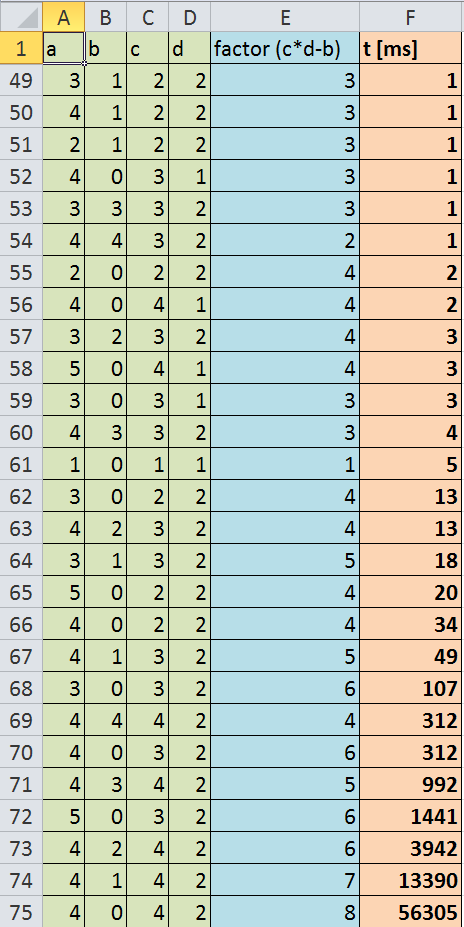
\includegraphics[width=0.80\textwidth]{excel.png}
\caption{Wyniki symulacji (pominięto pozycje z $t\approx0$)} 
\label{img:excel}
\end{figure}

Po agregacji wyników i posortowaniu ich po rosnącym czasie wykonania, na rysunku \ref{img:excel} widać, że podejrzenia, co do zależności złożoności obliczeniowej od ww. parametrów były słuszne. Wynika to z tego, że współczynnik oznaczony na rysunku jest w praktyce rozmiarem generowanych permutacji. Zważywszy na fakt, że w procesie generowania permutacji wyniki są także odpowiednio sortowane, aby zapewnić przejrzystość prezentacji uzyskanych rezultatów, można założyć, że osiągane czasy są zadowalające. Punktu ewentualnych poprawek można by poszukiwać w wykorzystanej zewnętrznej bibliotece generowania permutacji i próbie optymalizacji zagnieżdzonej pętli \texttt{for}. 

\begin{equation}
f(x)\in{O(\sum\limits_{i\in{\left\{A..N\right\}}}g(a_{i},b_{i},c_{i},d_{i}))} ,
\label{eqn:complexity}
\end{equation}
gdzie: $a$ to rozmiar alfabetu, $b$ to rozmiar ,,zbioru obowiązkowego'', $c$ to rozmiar markera a $d$ to liczba poszukiwanych osób.

\section{Języki i narzędzia}
Aplikacja została stworzona w języku Java w środowisku Eclipse\cite{eclipse}. Ze względu na wysoką przenośność, możliwość szybkiego jej przygotowania oraz bogate wbudowane biblioteki zdecydowaliśmy się na ten wybór. W toku pracy pomocne okazały się również zewnętrzne biblioteki \emph{combinatoricslib 2.0}\cite{combi} (biblioteka obiektów kombinatorycznych) oraz biblioteki do testów jednostkowych: główna - \emph{junit 4.11} wraz z \emph{hamcrest 4.11} odpowiedzialną za budowanie testów.

\section{Testowanie}
Testy aplikacji zostały wykonane za pomocą biblioteki JUnit. Przy pomocy testów jednostkowych zapewniliśmy, że wyniki zwracane przez aplikację są co do założeń zgodne, a \emph{test-driven development} pozwolił na wczesne wykrywanie ewentualnych problemów i pracę nad poszczególnymi funkcjonalnościami programu z bieżącą kontrolą postępu. Dzięki temu, przygotowanie wersji końcowej sprowadziło się w praktyce do złączenia testowanych metod w całość.

\section{Podsumowanie}
Podczas realizacji projektu mieliśmy okazję zapoznać się z problemem badania DNA dla celów kryminalistycznych od strony technicznej. Jak wspomniano na wstępie, przygotowany program spełnia z nawiązką wymagania określone w specyfikacji. Zdecydowaliśmy się jednak na implementację pozwalającą na wyznaczenie nieznanych profili dla dowolnej liczby osób. Niestety w parze z większą funkcjonalnością rozwiązania idzie dość duża złożoność obliczeniowa, o której wspomniano w punkcie \ref{badania}. Jak pokazano, w praktyce, dla n większego niż 10 czas działania programu potrzebny do uzyskania poprawnych wyników może być bardzo długi.

\begin{thebibliography}{9}

	\bibitem{eclipse} 
	\emph{Eclipse}\\
	\url{http://www.eclipse.org}
		
		\bibitem{combi}
	\emph{combinatoricslib -- biblioteka obiektów kombinatorycznych}\\
	\url{https://code.google.com/p/combinatoricslib/}

	\bibitem{junit}
	\emph{Junit -- framework testów jednostkowych}\\
	\url{http://junit.org}

	\bibitem{wikipedia}
	\emph{Wikipedia}\\
	\url{http://en.wikipedia.org/wiki/{DNA|DNA_marker|DNA_profiling}}
\end{thebibliography}
\end{document}
